\subsection{Test 2:}

Now let's encode a bigger file. As we can see in Figure 4.2.0, the {\itshape Original.txt} file has a lot of text, so, we will run the program and see what's in {\itshape Frequency.txt} and {\itshape Codification.txt} files ( Figures 4.2.1 and 4.2.2 ). \hfill \break

\begin{figure}[H]
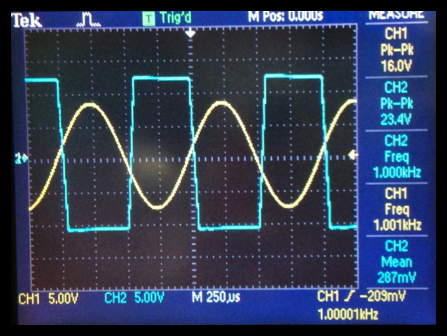
\includegraphics[height = 10cm, width = 16.5cm]{o2.png}
\centering \linebreak \linebreak Figure 4.2.0: Original.txt that store a {\bfseries C} program.
\end{figure} \hfill \break

\begin{multicols}{2}
\begin{figure}[H]
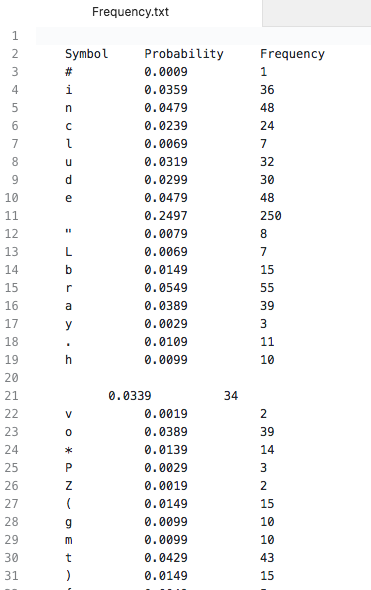
\includegraphics[height = 8cm, width = 6cm]{f2-1.png}
\centering
\end{figure} \hfill \break

\begin{figure}[H]
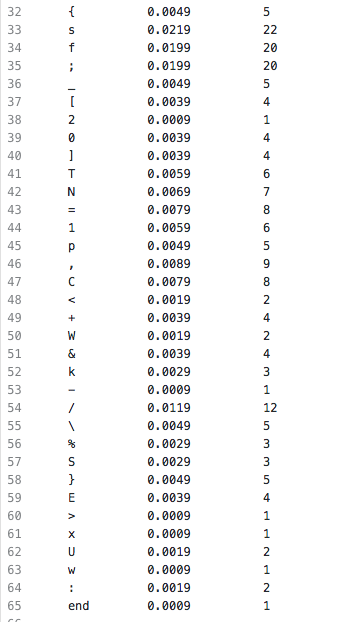
\includegraphics[height = 8cm, width = 6cm]{f2-2.png}
\centering
\end{figure} \hfill \break
\end{multicols}

\begin{center}
Figure 4.2.1: Frequency.txt file for Figure 4.2.0.
\end{center}

\begin{multicols}{2}
\begin{figure}[H]
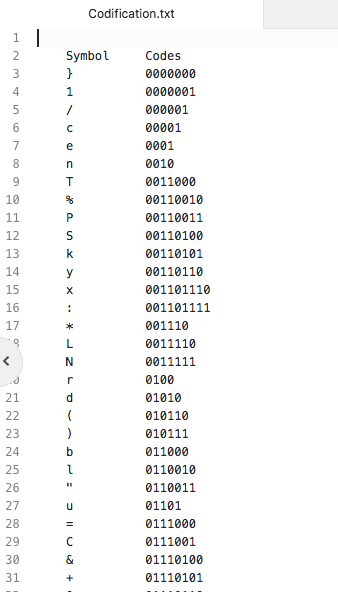
\includegraphics[height = 8cm, width = 6cm]{c2-1.png}
\centering
\end{figure} \hfill \break

\begin{figure}[H]
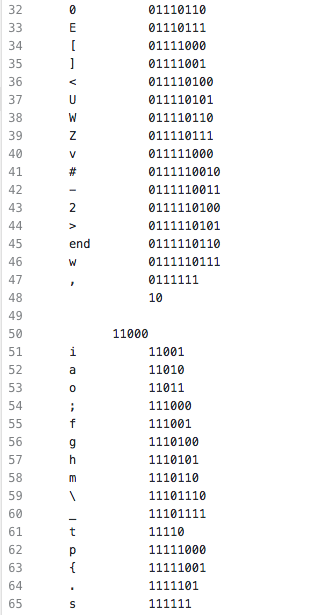
\includegraphics[height = 8cm, width = 6cm]{c2-2.png}
\centering
\end{figure} \hfill \break
\end{multicols} 

\begin{center}
Figure 4.2.2: Codification.txt file for Figure 4.2.0.
\end{center}

The output text or {\itshape binary-string} generated by the encoder program it's presented in Figure 4.2.3. \hfill \break

\begin{figure}[H]
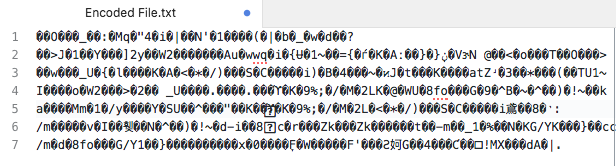
\includegraphics[height = 4cm, width = 16.5cm]{b2.png}
\centering \linebreak \linebreak Figure 4.2.3: Encoded File.txt 
\end{figure} \hfill \break

For decoding we run the program provided in the folder {\bfseries Decoder} that will take as parameters what ever it is in the file presented in Figure 4.2.3 and the dictionary of codes. Finally, after executing the decoding process, the program will generate a file named {\itshape Decoded File.txt}, as you can imagine, will store the decoded text. Figure 4.2.4 shows this output. \hfill \break

\begin{figure}[H]
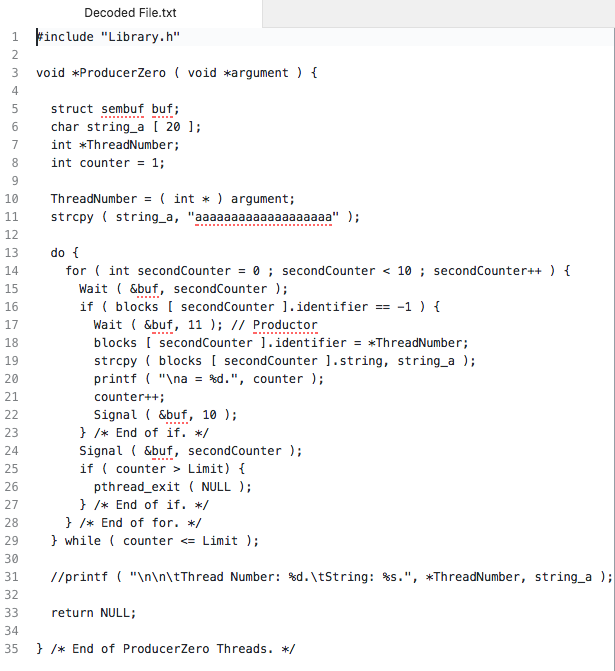
\includegraphics[height = 10cm, width = 16.5cm]{d2.png}
\centering \linebreak \linebreak Figure 4.2.4: Decoded File.txt
\end{figure} \hfill \break

Finally, to see if the encoder program actually really compress the size of {\itshape Original.txt} with the help of the {\itshape system information} we visualize that the size of this file it's bigger ( Figure 4.2.5 ) that the encoded one ( Figure 4.2.6 ). \hfill \break

\begin{multicols}{2}
\begin{figure}[H]
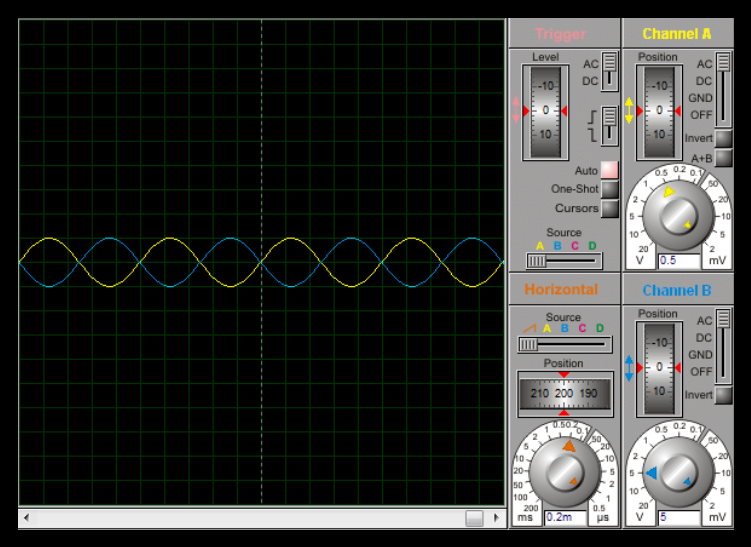
\includegraphics[height = 6cm, width = 6cm]{so1.png}
\centering \linebreak \linebreak Figure 4.2.5: Decoded file size.
\end{figure} \hfill \break

\begin{figure}[H]
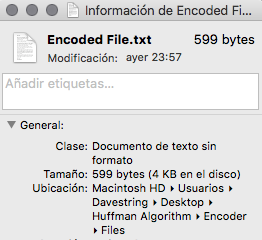
\includegraphics[height = 6cm, width = 6cm]{se2.png}
\centering \linebreak \linebreak Figure 4.2.6: Encoded file size.
\end{figure} \hfill \break
\end{multicols} 

As we can see the {\itshape Original.txt} file has a size of 1001 bytes in comparison with the Encoded one that has a size of 599 bytes.

\pagebreak